%!TEX root=main.tex
\section{Introduction} \label{intro}
From high-throughput genome sequencing, 
to multi-resolution astronomical imaging telescopes,
to at-scale physical testing of battery candidates,
many fields of science and engineering
are facing an increasing availability of 
large volumes of complex data~\cite{AustinNothaft2015,Demchenko2013},
holding the key to some of the most pressing 
unanswered scientific questions of our time,
such as: How does a treatment affect the 
expression of a gene in a breast cancer cell-line? 
Which battery components have sustainable levels 
of energy-efficiency and are safe and cheap to 
manufacture in production?  
While data analysis is central to a scientist's 
knowledge discovery process, scientists 
often lack the extensive experience to deal 
with data of this scale and complexity 
in a way that can facilitate rapid insight discovery~\cite{Kersten2011}. 

To explore their data, many scientists currently
create visualizations, either programmatically using 
tools (such as {\tt ggplot} or {\tt matplotlib}),
or visualization construction interfaces (such as 
Excel or Tableau)~\cite{Momcheva2015,Prabhu2011,Duck2016}. 
In either case, scientists are required to specify exactly what
they want to visualize. \tvcg{From early discussions with analysts from twelve different application areas, we learned that analysts often need to search for some desired pattern or trend amongst large numbers of visualizations.} For example, when trying to find celestial objects
corresponding to supernovae, which have a specific pattern
of brightness over time, scientists
need to individually \tvcg{inspect the visualizations of} each object (often numbering in the thousands) until they find ones that match the pattern. Similarly, when trying to infer relationships between two physical properties for different subsets of battery electrolytes, scientists need to individually visualize these properties
for each subset (out of an unbounded number of such subsets)
until they identify relationships that make sense to them. This process of manually exploring a large number of visualizations 
is \tvcg{not only error-prone, but also} overwhelming for scientists who do not have extensive knowledge about their
dataset. 
\par One potential solution for this challenge of manually exploring a large collection of visualizations
are systems that allow users to specify 
desired visual patterns, via a high-level specification language
or interface, with the system automatically
traversing all potential visualization candidates to find
and return those that match the specification. 
We define such systems to be {\em Visual Query Systems}, or VQSs for short.
There are a number of VQSs that have been introduced in the literature~\cite{mohebbi2011google,Hochheiser2004,wattenberg2001sketching,Siddiqui2017VLDB,ryall2005querylines,holz2009relaxed}. 
\tvcg{For example, Google Correlate~\cite{mohebbi2011google} 
and QuerySketch~\cite{wattenberg2001sketching} allow users to draw a trend of interest, with the system automating the search to find matching visualizations.}
\par \tvcg{Not surprisingly, when asked about the potential viability of VQSs in aiding scientific data analysis,  many scientists indicated that VQSs could be useful in mitigating the challenge of visualization exploration described earlier---since it automates the painful manual exploration of visualizations to find desired patterns.}
Yet, to the best of our knowledge, 
VQSs are not very commonly used in practice.
{\em Our paper seeks to bridge this gap between current research on VQSs \tvcg{to understand why existing VQSs are not commonly used by analysts} and how they can actually be used in practice, as a first step towards the broad adoption of VQSs in data analysis}. 
In this paper, we present findings from a series of interviews, cognitive walkthroughs, participatory design, and user studies with scientists from three different scientific 
domains---{\em astronomy, genetics,} and {\em material science}---through a year-long collaboration.
These scientific use cases present a diverse set of goals and datasets that could benefit from a VQS. Our three main research questions are as follows:
\par \emph{RQ1: What are the challenges in existing scientific data analysis workflows that could be potentially addressed by a VQS?}

Via cognitive walkthroughs and interviews,
we gained an understanding of the data analysis 
workflows presently employed by the scientists, their needs,
and the challenges they face. 
We identified opportunities where a VQS could
help accelerate their analysis, by helping them
discover insights, gain intuition, or provoke directions
for exploration. Finally, we determined the types of 
research questions and dataset properties that would
be most suitable for exploration on VQSs.
%By learning about the needs and challenges that scientists face when working with their datasets through interviews and cognitive walkthroughs, we learned about the types of queries that they would like to pose on VQSs and distilled a set of design specifications that can better enable VQSs to help them discover insights, gain intuition about their datasets or provoke further directions for exploration. We also identify the types of research questions and dataset properties would be suitable for data exploration on VQSs.
\begin{figure*}[ht!]
\centering
\vspace{-15pt}
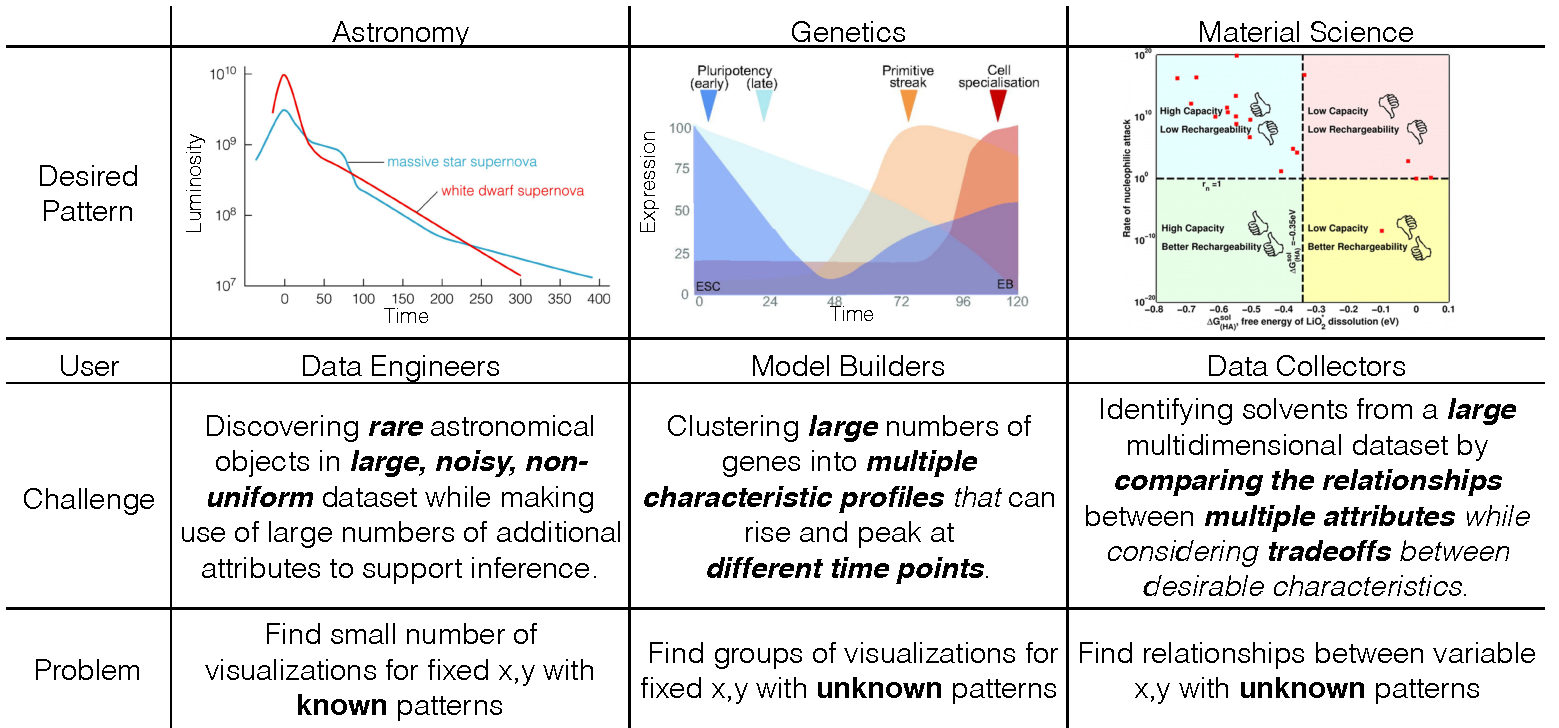
\includegraphics[width=0.8\linewidth]{figures/sci_challenge_tbl.pdf}
\vspace{-6pt}\caption{Descriptions of the three scientific use cases discussed in this paper.}
\label{example}
\vspace{-10pt}
\end{figure*}

\par\emph{RQ2: What types of interface capabilities are necessary to develop VQSs into a useful component of data analysis?}

Via participatory design, we distilled a set of key features that our scientist participants would
need for VQSs to be useful and usable within their data analysis workflows. 
\tvcg{Based on our early interactions with scientists, 
we started to build a VQS~\cite{Siddiqui2017VLDB,Siddiqui2017} that, similar to existing VQSs~\cite{wattenberg2001sketching}, allowed them to search for desired trends via drawing on a canvas. This early system served as a functional prototype for us to engage with scientists further in a participatory design process, understand how they envision themselves using a VQS, and gather feedback on feature designs that could make the VQS more useful. The features we developed address challenges shared across the three scientific domains, ranging from additional querying modalities, to features that support a more integrated workflow, to improving the interpretability of the system output, not all of which were supported by prior VQSs in the literature. Our collaborative design experience culminated in a full-fledged VQS, \zv, capable of facilitating rapid hypothesis generation and insight discovery.}

\emph{RQ3: How do VQSs accelerate scientific insights?}\\
\emph{RQ4: How can VQSs fit within the context of existing data analysis workflows?}
\\ To evaluate our final system \zv, we conducted a user study with nine scientists (including those who had participated in the design process), all of whom had a vested interest in using a VQS to address their research questions on their datasets. In a 1.5-hour user study, our scientist participants were able to gain novel scientific insights, such as \emph{\tvcg{identifying a star with a transit pattern that was known to harbor a Jupiter-sized planet,} finding characteristic gene expression profiles that confirmed the results of a related publication, and learning that the dip in an astronomical light curve is caused by saturated imaging equipment overlooked by the existing error-flagging pipeline}.  Participants also gained additional insights about their datasets, including debugging \tvcg{mislabelled features and 
uncovering the erroneous data preprocessing procedure applied to a collaborator's dataset.}
% that the way data is aggregated across multiple experiments is erroneous on a collaborator's dataset. 
We learned how VQSs could be contextualized within scientific data analysis workflows and discovered that VQSs can be used beyond the exploratory phase of analysis, for data verification, debugging preliminary datasets, and performing sanity-checks on downstream models.
\par As most existing VQSs are evaluated in a standalone fashion via artificial tasks and datasets, to the best of our knowledge, \emph{our study is the first to holistically examine how VQSs can be used in practice and integrated into existing data analysis workflows}. From these experiences, we advocate common design guidelines and end-user considerations when building the next generation VQSs.